\section{Introducción}
En los capítulos anteriores realicé una revisión del estado del arte sobre el \textit{graph mining} aplicado en el área de la salud, con las definiciones en las cuales se enmarca esta tesis. Además, describí el proceso de ETL para obtener el conjunto de datos que constituye el grafo de la lista de problemas con sus relaciones a SNOMED CT, el cual es un grafo dirigido acíclico.

En éste capítulo realizaré experimentos sobre el grafo, dividiéndolo en dos versiones, la primera con las relaciones a SNOMED CT, y la segunda sin las relaciones. En capítulos anteriores se mostró inconsistencias entre los conceptos de la red de SNOMED CT, donde conceptos muy similares estaban muy distantes y conceptos muy distintos estaban muy cerca, es de interés analizar si las conexiones de SNOMED mejoran la capacidad de formar comunidades y la capacidad predictiva de los modelos.

En la primera parte de este capítulo aplicaré las definiciones de los grafos descriptas en los capítulos anteriores, evaluando si los grafos formados siguen patrones de red. 

La segunda parte contiene el análisis sobre los agrupamientos encontrados luego de aplicar los algoritmos \textit{label propagation}, \textit{leading vector} y \textit{multilevel}. Las red creada sólo a partir de los problemas y sus conexiones será enriquecida con información sobre el nivel asistencial, grupo etáreo y servicio de salud en el cuál el problema fue seleccionado. 

Además de describir los resultados obtenidos y los outliers encontrados, se evaluará la capacidad predictiva de los conceptos que están en el mismo grupo dada una lista de problema de un paciente.

\section{Definición del grafo}
Sea el grafo de la figura\ref{fig:ModeloGrafo} G=(V,E), donde V denota a los vértices, equivalente a nodos: conceptos de snomed CT y pacientes, y E denota las aristas, equivalente a relaciones: \textit{tiene un problema}, o conexiones jerárquicas $|\textit{is a}|$ (Hallazgo Clínico, Procedimientos, Eventos, Situación con contexto explícito). Los \num{88869} conceptos distintos de la lista de problemas están relacionados jerárquicamente con \num{11946} de snomed, de tal manera que al usar todos los conceptos de las jerarquías, el número de vértices y aristas de la red son $|V|=$\num{19354} y $|E|=$\num{1173234} respectivamente. Las aristas de la red son ponderadas por la frecuencia de ocurrencia del problema en el paciente. 

De manera paralela, realizo el análisis sobre el subgrafo generado sólo con las relaciones \textit{tiene un problema} y los nodos que comparten esta relación. El número de vértices y aristas de este subgrafo son $|V|=$\num{11946} y $|E|=$\num{937107} respectivamente.

Para diferenciar las dos redes, la primera la nombro como \textbf{Red semántica de problemas(RSP)} y la segunda la nombro como \textbf{Red de problemas(RP)}

\begin{figure}[ht]
\caption{Modelo de datos de grafos de la lista de problemas}
\label{fig:ModeloGrafo}
\centering
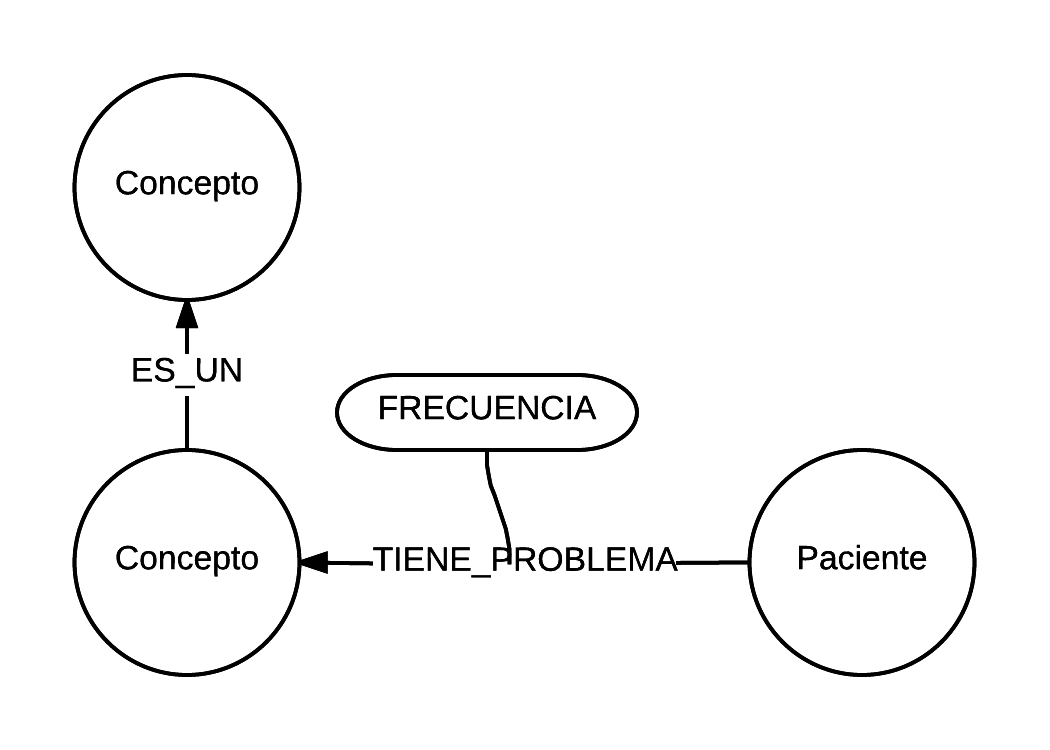
\includegraphics[width=0.6\textwidth]{Modelo_grafo_}
\end{figure}

\section{Patrones de la red de la lista de problemas}
\subsubsection{Red libre de escala}
En esta sección evalúo si la redes comparte patrones con redes de gran escala, realizo un ajuste a una distribución de ley de potencias usando los grados de cada nodo, con la $H0:$ los datos se distribuyen según la ley de potencias, y estimo la función de distribución acumulativa (cdf). Si el p-value no permite rechazar la hipótesis nula otra estrategia para determinar la distribución de los datos es comparar el estadístico \textit{log-likelihood ratio} con otras dos distribuciones, el resultado es positivo si los datos se ajustan más a la primera distribución, y negativa si los datos son más como la segunda distribución.

En el caso de la \textbf{RSP} la función cdf es:
\begin{equation}
F(X\geq 51) \propto x^{-1.82 +1}
\end{equation}

Dado que el p-value$(0.3188>0.05)$ no me permite rechazar la hipótesis nula, realizo la comparación con otras distribuciones. En la tabla \ref{distribucion} están los resultados de las comparaciones realizadas entre ley de potencias con otras distribuciones: la distribución exponencial fue usada para confirmar que los datos tienen una cola pesada, y la distribución lognormal tiene un mejor ajuste que la ley de potencias, como se muestra también en la figura \ref{fig:ajusteDistribuciones}.

% Please add the following required packages to your document preamble:
% \usepackage{booktabs}
\begin{table}[htb]
\centering
\caption{Comparación de la ley de potencias con otras distribuciones de la red semántica de problemas}
\label{distribucion}
\begin{threeparttable}
\begin{tabular}{@{}lr@{}}
\toprule
Distribución & Resultado    \\ \midrule
Exponencial  & 10.64\tnote{*}  \\
Lognormal    & -1.5 \\ \bottomrule
\end{tabular}
\begin{tablenotes}
    \item[*] p-value$<$\num{0.05}.
  \end{tablenotes}
\end{threeparttable}
\end{table}

\begin{figure}[ht]
\caption{Gráfico log-log, comparación de ajuste de distribuciones de la red semántica de problemas}
\label{fig:ajusteDistribuciones}
\centering
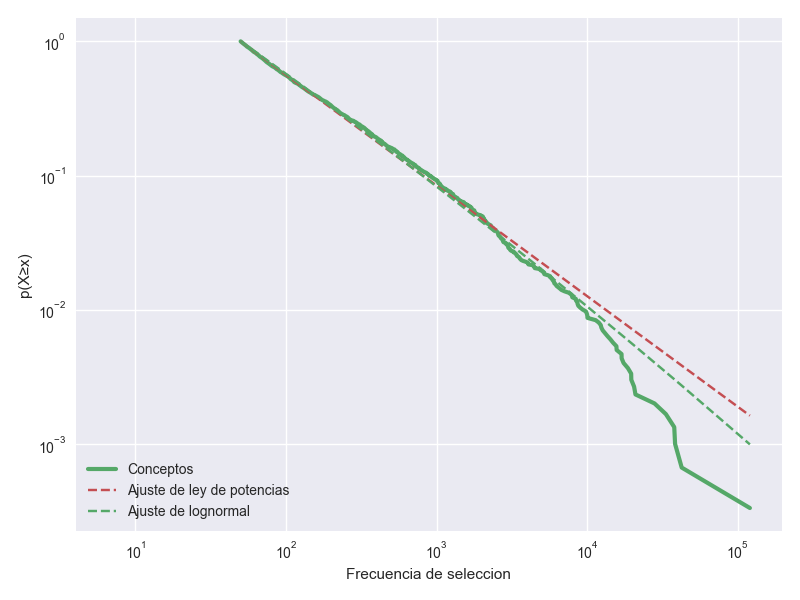
\includegraphics[width=0.6\textwidth]{chart6}
\end{figure}

En el caso de la \textbf{RP} la función cdf es:
\begin{equation}
F(X\geq 279) \propto x^{-1.86 +1}
\end{equation}

Dado que el p-value$(0.03<0.05)$ se acepta la hipótesis $H0:$ los datos se distribuyen según la ley de potencias. La figura \ref{fig:ajusteDistribucionesRP} muestra también que esta distribución tiene mejor ajuste.

\begin{figure}[ht]
\caption{Gráfico log-log, comparación de ajuste de distribuciones de la red de problemas}
\label{fig:ajusteDistribucionesRP}
\centering
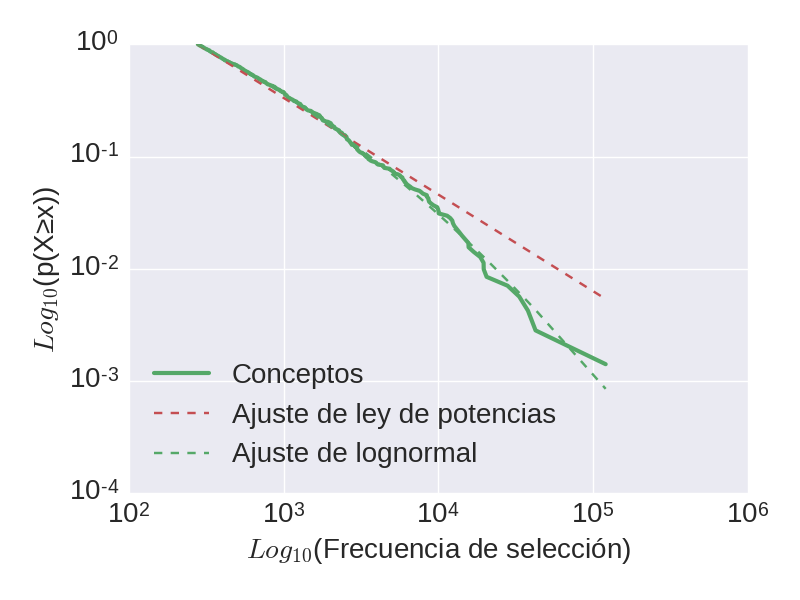
\includegraphics[width=0.6\textwidth]{chart7}
\end{figure}

% fit.distribution_compare('power_law', 'exponential', normalized_ratio = True)
%(4.6415121033253648, 3.4586875833842345e-06)
%>>> fit.distribution_compare('power_law', 'lognormal', normalized_ratio = True)(-2.4059692368632613, 0.016129622892949523)

\subsubsection{Fuertes estructuras de comunidad}
Existen diferentes métricas para evaluar cuantitativamente los efectos de comunidad en un grafo, las usadas  a continuación siguen el trabajo de Boccaletti \textit{et. al}\cite{BOCCALETTI2006} y están disponibles en los paquetes igraph\cite{igraph} y netowrkx\cite{SciPyProceedings_11} de python.

\begin{table}[htb]
\centering
\caption{Métricas de efectos de comunidad en redes}
\label{community-graphs}
\resizebox{\textwidth}{!}{%
\begin{tabular}{@{}lrr@{}}
\toprule
Métrica                                                  & Valor en la RSP  & Valor en la RP            \\ \midrule
Coeficiente de agrupamiento - transitividad                & \num{0.19} & \num{0.21} \\
Coeficiente de agrupamiento - transitividad local promedio & \num{0.41}  & \num{0.80}\\
Coeficiente de agrupamiento promedio                        & \num{0.34}  & \num{0.78}      \\
Longitud media del camino mínimo entre nodos             & \num{2.80}  & \num{2.17}  \\
Promedio de grados                                       & \num{60.62}  & \num{78.4}      \\ \bottomrule
\end{tabular}%
}
\end{table}

La diferencia de las métricas de transitividad y la transitividad local promedio, es que la primera es la medida de la transitividad local en toda la red, en la segunda se calcula por cada vértice la transitividad y los nodos con menos de dos vecinos son considerados como de transitividad cero\cite{Watts1998}. Las diferencias entre estas dos métricas indican una alta presencia de nodos que no forman tríadas.

Los valores de coeficiente de agrupamiento cercanos a 1 indican alto grado de agrupamiento, como se puede ver en la tabla \ref{community-graphs} la \textbf{RP} tiene mejores coeficientes que la \textbf{RSP}. 

Aunque los valores de la longitud media del camino mínimo entre nodos entre las dos redes es similar, para un alto coeficiente de agrupamiento como es el caso de \textbf{RP} el efecto es que la mayoría de los nodos que son homogéneos se encuentran en pocos saltos dentro de la red, este efecto es similar al fenómeno de mundo pequeño en las redes sociales\cite{Cook2006}. Además, estos nodos tienen en promedio más nodos vecinos que la \textbf{RSP}.

\section{Agrupamiento}

Apliqué los algoritmos de agrupamiento: \textit{label propagation}, \textit{leading vector} y \textit{multilevel} a el grafo de la \textbf{RP} y a sub-grafos de la \textbf{RSP}, conformados por relaciones que tengan un mínimo de frecuencia en pacientes (\num{5}, \num{10}, \num{100}, \num{1000} y \num{10000}). Esto con el propósito de evaluar la estabilidad de los agrupamientos aunque el grafo pierda nodos.

La tabla \ref{res_agru} contiene los resultados de los coeficientes de agrupamiento para cada grafo y la cantidad de grupos encontrados. Se puede observar que en el caso del grafo de la \textbf{RP} se generan similares número de grupos aunque el coeficiente de clustering varía en los algoritmos. El más alto coeficiente es el del algoritmo \textit{multilevel} y el más bajo es el de \textit{label propagation}, aunque estos dos son algoritmos aglomerativos el primero optimiza la ganancia en la función de modularidad, mientras que el segundo realiza un consenso entre los nodos de un mismo grupo para decidir el grupo al que pertenecen todos.

En el caso de los grafos \textbf{RSP}, el número de grados varía entre algoritmos, \textit{multilevel} es también el que mejores coeficientes obtiene y mientras que \textit{leading vector} va desmejorando en sus coeficientes a medida que crece el grafo, \textit{label propagation} mejora. \textit{leading vector} es un algoritmo divisivo que se ve afectado por el tamaño del grafo y \textit{label propagation} va hallando estructuras más cohesivas en la medida que crece el grafo.


% Please add the following required packages to your document preamble:
% \usepackage{booktabs}
% \usepackage{multirow}
% \usepackage{graphicx}
\begin{table}[htb]
\centering
\caption{Resultados de agrupamiento de grafos de problemas}
\label{res_agru}
\resizebox{\textwidth}{!}{%
\begin{tabular}{@{}lrrrrrr@{}}
\toprule
\multirow{3}{*}{Grafo}                                                                                          & \multicolumn{6}{l}{Algoritmos de clasifcación}                                                                                                                                             \\ \cmidrule(l){2-7} 
                                                                                                                & \multicolumn{2}{l}{Leading Vector}                           & \multicolumn{2}{l}{Multilevel}                               & \multicolumn{2}{l}{Label Propagation}                        \\ \cmidrule(l){2-7} 
                                                                                                                & \multicolumn{1}{l}{Coeficiente} & \multicolumn{1}{l}{Grupos} & \multicolumn{1}{l}{Coeficiente} & \multicolumn{1}{l}{Grupos} & \multicolumn{1}{l}{Coeficiente} & \multicolumn{1}{l}{Grupos} \\ \cmidrule(r){1-7}
Red de Problemas(RP)                                                                                                & 0.36                            & 22                         & 0.43                            & 23                         & 0.08                            & 22                         \\
\begin{tabular}[c]{@{}l@{}}Red Semántica de Problemas \\ (Relaciones en al menos 10000 individuos)\\(RSP-10.000)\end{tabular} & 0.50                            & 14                         & 0.59                            & 27                         & 0.27                            & 87                         \\
\begin{tabular}[c]{@{}l@{}}Red Semántica de Problemas \\ (Relaciones en al menos 1000 individuos)\\(RSP-1.000)\end{tabular}  & 0.50                            & 14                         & 0.59                            & 27                         & 0.27                            & 88                         \\
\begin{tabular}[c]{@{}l@{}}Red Semántica de Problemas \\ (Relaciones en al menos 100 individuos)\\(RSP-100) \end{tabular}   & 0.50                            & 14                         & 0.59                            & 24                         & 0.29                            & 92                         \\
\begin{tabular}[c]{@{}l@{}}Red Semántica de Problemas \\ (Relaciones en al menos 10 individuos)\\(RSP-10) \end{tabular}    & 0.29                            & 11                         & 0.61                            & 24                         & 0.37                            & 91                         \\
\begin{tabular}[c]{@{}l@{}}Red Semántica de Problemas \\ (Relaciones en al menos 5 individuos)\\(RSP-5)\end{tabular}     & 0.32                            & 12                         & 0.62                            & 25                         & 0.46                            & 88                         \\ \bottomrule
\end{tabular}%
}
\end{table}

Estos seis grafos con sus 3 algoritmos representan grupos fuertes y débiles, a continuación presento los grupos de problemas que son consistentes en todos los agrupamientos. Además calculo la longitud media del camino mínimo entre los nodos del agrupamiento, medida que es usada como distancia semántica en diferentes trabajos en el dominio médico\cite{Wang2010TheAudit.,Gan2013,Pedersen2007,Zare2015ASNOMED-CT}. Esta información permite detectar grupos con conceptos con diferentes significados semánticos y outliers.

\subsection{Agrupamientos de Red de Problemas (RP)}
Combinando los resultados de los agrupamientos hay \num{11132} posibles combinaciones, encontré 53 grupos de problemas que comparten las mismas agrupaciones. Según la tabla, \ref{gruposRP} la mayoría (19) de los grupos encontrados tienen 2 nodos, los grupos que tiene más nodos tienen en promedio una mediana de grados por nodo más grande, es decir que son nodos altamente conectados.

Al analizar las distancias semánticas entre los conceptos que comparten el mismo grupo, puedo observar según la figura \ref{fig:bpDistanciasSemanticasRP} que la mayoría de las medianas de las distancias se ubican cercanas a 10. Los casos con las mayores dispersiones son el cluster\_1, cluster\_6, cluster\_10, cluster\_16, cluster\_22, cluster\_27, cluster\_30, cluster\_34 y cluster\_36. 

En la tabla \ref{top10_rp} se encuentra el top 10 de los conceptos por agrupamiento según diferentes métricas de centralidad (grado, cercanía e intermediación). En esta tabla se encuentran sólo los casos de las mayores dispersiones, el top 10 según el grado y la cercanía es muy similar en la mayoría de los casos; difiere en el caso de la intermediación, donde se pueden encontrar nodos que sin tener muchas conexiones son mucho más importantes para la conexión de otros dos nodos.

Por ejemplo, según lo anterior en el caso del cluster\_6 (que se puede interpretar como de enfermedades generales), los problemas con mayor grado (los más populares) son: FIEBRE y TOS, pero el problema con mayor intermediación es RESFRIÓ COMÚN. Es decir, que este último conecta más otros pares de problemas que la Fiebre y la Tos. Otros ejemplos se pueden encontrar en el cluster\_10, donde el problema con mayor grado y cercanía es MALESTAR GENERAL, y el de mayor intermediación es INMUNODEFICIENCIA COMBINADA SEVERA; en el grupo de embarazo (cluster\_16) donde los problemas con mayor grado son PACIENTE ACTUALMENTE EMBARAZADA, ANSIEDAD y MAREO, pero los de mayor intermediación son AMENAZA DE TRABAJO DE PARTO PREMATURO, INTOXICACIÓN POR FÁRMACO Y/O SUSTANCIA MEDICINAL y SANGRADO VAGINAL.

\subsubsection{outliers}
Según el boxplot generado con las distancias semánticas en la figura \ref{fig:bpDistanciasSemanticasRP}, se presentan outliers en los siguientes clusters:
\begin{itemize}
\item cluster\_6: Este es un agrupamiento de enfermedades generales donde los problemas que tiene mayor distancia semántica en promedio con el resto del mismo grupo es: CIRUGÍA DE CATARATAS(PROCEDIMIENTO), ATAQUE DE PÁNICO(HALLAZGO), AMIGDALECTOMÍA(PROCEDIMIENTO)
\item cluster\_10: Este es un agrupamiento de administración de medicamentos y procedimientos invasivos, los problemas con mayores distancias son: ADMINISTRACIÓN DE ANTICOAGULANTE(PROCEDIMIENTO), TRATAMIENTO CON ANTIBIÓTICOS INTRAVENOSOS(PROCEDIMIENTO), INYECCIÓN DE GAMMAGLOBULINA (PROCEDIMIENTO), CAMBIO DEL TUBO DE TRAQUEOSTOMÍA (PROCEDIMIENTO). Estas distancias se explican porque la mayoría de los conceptos de este grupo están en la jerarquía de Hallazgos.
\item cluster\_27: En este agrupamiento de enfermedades relacionadas con la edad avanzada, los problemas que tienen mayor distancia son: CONFUSIÓN AGUDA(HALLAZGO), PACIENTE EN CAMA (HALLAZGO).
\item cluster\_36: En este agrupamiento de enfermedades cardiopulmonares, las mayores distancias se encuentran en los siguientes conceptos: BIOPSIA ENDOMIOCÁRDICA (PROCEDIMIENTO), ALOTRASPLANTE ORTOTÓPICO DE CORAZÓN (PROCEDIMIENTO) y TUMOR DE KLATSKIN (TRASTORNO), esta última considerada como una enfermedad huérfana\footnote{www.orpha.net/consor/cgi-bin/OC\_Exp.php?lng=ES\&Expert=99978}.
\end{itemize}

Los outliers en las cotas inferiores se debe a relaciones de especificación entre conceptos, por ejemplo: en el cluster\_42: EPISTAXIS ANTERIOR es descendiente de EPISTAXIS, y ambos conceptos están en el mismo grupo.

% Please add the following required packages to your document preamble:
% \usepackage{booktabs}
\begin{table}[htb]
\centering
\caption{Grupos que comparten las mismas agrupaciones en la red de problemas}
\label{gruposRP}
\begin{tabular}{@{}rrr@{}}
\toprule
Número de Nodos & Grupos Encontrados & Mediana de grados por nodo \\ \midrule
2               & 19                 & 1949                       \\
3               & 9                  & 1832                       \\
4               & 5                  & 1833                       \\
5               & 1                  & 1818                       \\
6               & 5                  & 3287                       \\
7               & 1                  & 1590                       \\
8               & 2                  & 5192                       \\
10              & 2                  & 2222                       \\
13              & 1                  & 802                        \\
16              & 1                  & 990                        \\
22              & 1                  & 2198                       \\
25              & 1                  & 3008                       \\
34              & 1                  & 4210                       \\
45              & 1                  & 864                        \\
59              & 1                  & 3700                       \\
77              & 1                  & 1228                       \\
84              & 1                  & 3234                       \\ \bottomrule
\end{tabular}
\end{table}

\begin{figure}[ht]
\caption{Distancias semánticas entre conceptos del cluster}
\label{fig:bpDistanciasSemanticasRP}
\centering
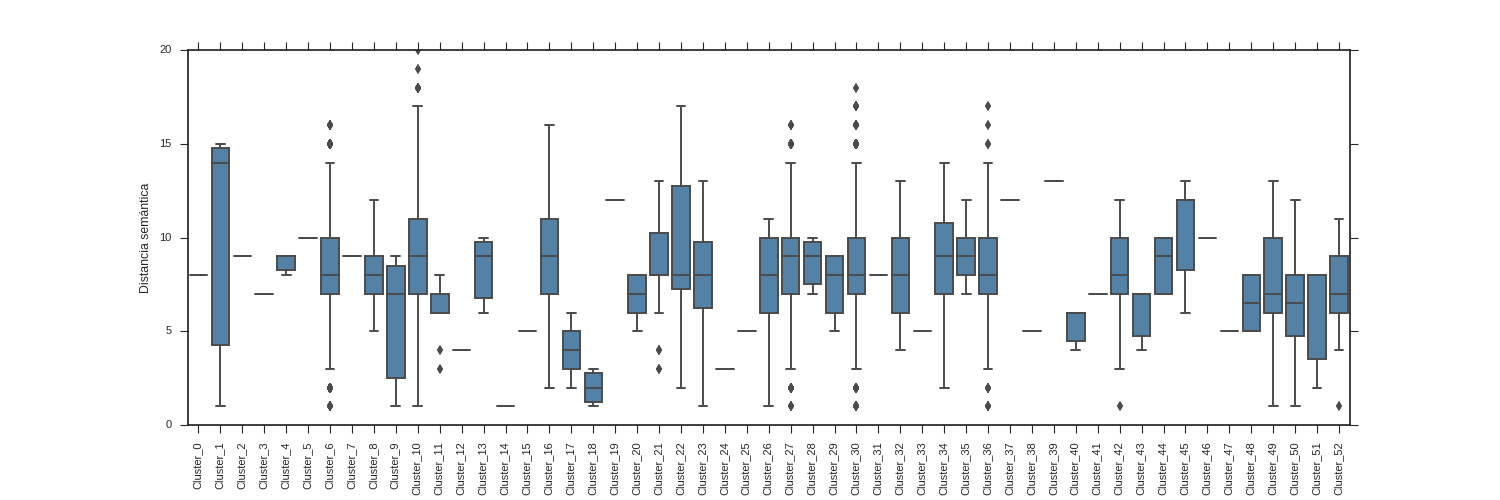
\includegraphics[width=\textwidth]{bpDistanciasSemanticasRP}
\end{figure}

\subsection{Agrupamientos de Red Semántica de Problemas (RSP)}
Combinando los resultados de los agrupamientos hay \num{2,39e26} posibles combinaciones, encontré 68 grupos de problemas que comparten las mismas agrupaciones. Según la tabla \ref{gruposRSP} La mayoría (44) de los grupos encontrados tienen 2 nodos.

Al analizar las distancias semánticas entre los conceptos que comparten el mismo grupo, puedo observar según la figura \ref{fig:bpDistanciasSemanticasRSP} que las medianas de las distancias tienen un mínimo de 1 y máximo de 10, y no presentan una tendencia. 

En la tabla \ref{top10_rsp} se encuentra el top 10 de los conceptos por agrupamiento según diferentes métricas de centralidad (grado, cercanía e intermediación). Estos grupos son más pequeños que el caso anterior, pero sobresalen los grupos con distancias semánticas grandes cuyos conceptos pareciera que no están muy relacionados, por ejemplo, el cluster\_0: INCISIÓN DE LA TRÁQUEA, AMIGDALECTOMÍA y CIRUGÍA DE CATARATAS, el cluster\_2: FÍSTULA TRAQUEOESOFÁGICA y ÚTERO UNICORNE, el cluster\_6: HIPERCORTISOLISMO y TUMOR DE KLATSKIN, pero al hacer una búsqueda rápida se pueden encontrar evidencias de las relaciones de estas enfermedades en artículos de divulgación científica, como se muestra en la tabla \ref{evidencia_grupos_2}.

\subsubsection{outliers}
Según el boxplot generado con las distancias semánticas en la figura \ref{fig:bpDistanciasSemanticasRSP}, se presentan outliers sólo en el cluster\_56 formado por: PROCTORRAGIA, INDIGESTIÓN, DISFAGIA, VEJIGA: INCONTINENTE, CÁLCULO RENAL, HEMORRAGIA DIGESTIVA BAJA, SÍNDROME DE ICTERICIA COLESTÍSICA y PIELONEFRITIS. Los problemas con mayores distancias son VEJIGA: INCONTINENTE y SÍNDROME DE ICTERICIA COLESTÍSICA


% Please add the following required packages to your document preamble:
% \usepackage{booktabs}
\begin{table}[htb]
\centering
\caption{Grupos que comparten las mismas agrupaciones en la red semántica de problemas}
\label{gruposRSP}
\begin{tabular}{@{}rrr@{}}
\toprule
Número de Nodos & Grupos Encontrados & Mediana de grados por nodo \\ \midrule
2	& 44	&2041 \\
3	&12 &	2144\\
4	&3&	1843\\
5	&4&	1826\\
6	&2&	1226\\
8	&2&	3501\\
9	&1&	1172                   \\ \bottomrule
\end{tabular}
\end{table}

\begin{figure}[ht]
\caption{Distancias semánticas entre conceptos del cluster}
\label{fig:bpDistanciasSemanticasRSP}
\centering
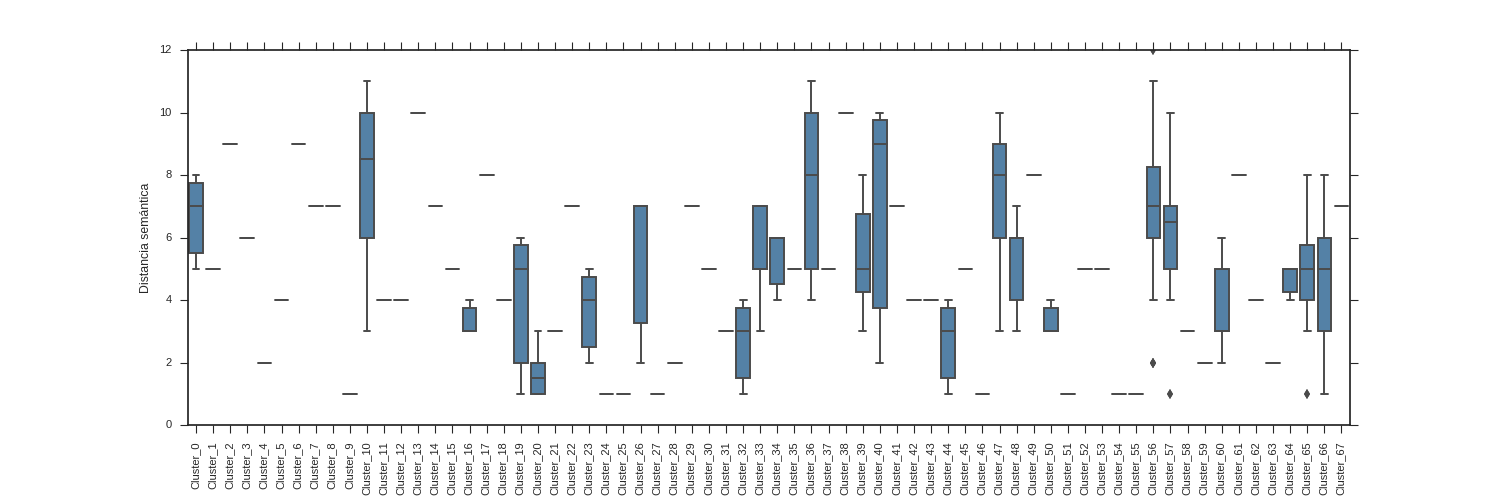
\includegraphics[width=\textwidth]{bpDistanciasSemanticasRSP}
\end{figure}

\subsubsection{Agrupamientos \textit{Label Propagation}}
Combinando los resultados de aplicar el algoritmo \textit{label propagation} en la RSP con diferentes cantidades mínimas de individuos que tengan el problema, hay \num{5.64e9} posibles combinaciones y encontré 232 grupos comunes a todos los resultados de agrupamiento. 

Según los resultados obtenidos, resumidos en la tabla \ref{clus_lp}, más del 50\% de los grupos tienen menos de 50 nodos, estos grupos son muy cohesivos, ya que tienen distancias en promedio de dos saltos entre nodos y con una baja cantidad total de distancias outliers entre los nodos (10 en total en 144 grupos). Los grupos más grandes tienen también la mayor cantidad de distancias outliers, se presentó el caso de los clusters 18 y 215 con \num{15083524} y \num{894907} número de distancias entre nodos respectivamente, y entre los dos suman más de \num{6600} distancias outliers.

% Please add the following required packages to your document preamble:
% \usepackage{booktabs}
% \usepackage{graphicx}
\begin{table}[htb]
\centering
\caption{Agrupamientos con el algoritmo \textit{Label propagation}}
\label{clus_lp}
\resizebox{\textwidth}{!}{%
\begin{tabular}{@{}lrrrrrr@{}}
\toprule
Número de nodos & \multicolumn{1}{l}{\begin{tabular}[c]{@{}l@{}}Número de \\ agrupamientos\end{tabular}} & \multicolumn{1}{l}{\begin{tabular}[c]{@{}l@{}}Promedio de mediana \\ de distancias \\ entre nodos\end{tabular}} & \multicolumn{1}{l}{\begin{tabular}[c]{@{}l@{}}Desviación estándar\\ de Mediana de distancias \\entre nodos\end{tabular}} & \multicolumn{1}{l}{\begin{tabular}[c]{@{}l@{}}Mediana  máxima \\de distancias \\entre nodos\end{tabular}}  & \multicolumn{1}{l}{\begin{tabular}[c]{@{}l@{}}Mediana mínima \\de distancias \\entre nodos\end{tabular}} & \multicolumn{1}{l}{\begin{tabular}[c]{@{}l@{}} Distancias Outliers\\ entre todos los\\ agrupamientos\end{tabular}} \\ \midrule
Menores de 50 nodos & 144 & 2 & 1,7 & 10 & 1 & 10 \\
Entre 50 y 100 nodos & 25 & 2 & 0,8 & 5 & 2 & 34 \\
Entre 100 y 200 nodos & 13 & 3 & 1,4 & 8 & 2 & 0 \\
Entre 200 y 500 nodos & 20 & 3 & 1,1 & 7 & 2 & 56 \\
Entre 500 y 1000 nodos & 10 & 4 & 1,4 & 7 & 3 & 106 \\ 
Mayor de 1000 nodos & 20 & 6 & 1,4 & 9 & 4 & 6600 \\\bottomrule
\end{tabular}%
}
\end{table}

\subsubsection{Agrupamientos \textit{Leading vector}}
Combinando los resultados de aplicar el algoritmo \textit{Leading Vector} en la RSP con diferentes cantidades mínimas de individuos, hay \num{3.62e5} posibles combinaciones y encontré 38 grupos comunes a todos los resultados de agrupamiento.

Según la tabla \ref{clus_lv}, el 50\% de los agrupamientos tienen más de 1000 nodos. El resto de los grupos son bastante cohesivos, con distancias promedios cercanas a 3 y sin distancias outliers.

\begin{table}[htb]
\centering
\caption{Agrupamientos con el algoritmo \textit{Leading vector}}
\label{clus_lv}
\resizebox{\textwidth}{!}{%
\begin{tabular}{@{}lrrrrrr@{}}
\toprule
Número de nodos & \multicolumn{1}{l}{\begin{tabular}[c]{@{}l@{}}Número de \\ agrupamientos\end{tabular}} & \multicolumn{1}{l}{\begin{tabular}[c]{@{}l@{}}Promedio de mediana \\ de distancias \\ entre nodos\end{tabular}} & \multicolumn{1}{l}{\begin{tabular}[c]{@{}l@{}}Desviación estándar\\ de Mediana de distancias \\entre nodos\end{tabular}} & \multicolumn{1}{l}{\begin{tabular}[c]{@{}l@{}}Mediana  máxima \\de distancias \\entre nodos\end{tabular}}  & \multicolumn{1}{l}{\begin{tabular}[c]{@{}l@{}}Mediana mínima \\de distancias \\entre nodos\end{tabular}} & \multicolumn{1}{l}{\begin{tabular}[c]{@{}l@{}}Distancias Outliers\\ entre todos los\\ agrupamientos\end{tabular}} \\ \midrule
Menores de 50 nodos & 15 & 3,4 & 2,8 & 9 & 1 & 0 \\
Entre 50 y 100 nodos & 3 & 3 & 1,7 & 5 & 2 & 0 \\
Entre 100 y 200 nodos & 1 & 3 & - & 3 & 3 & 0 \\
Entre 500 y 1000 nodos & 2 & 5,5 & 0,7 & 6 & 5 & 0 \\
Mayor de 1000 nodos & 19 & 7 & 1,2 & 9 & 5 & 50712 
\\\bottomrule
\end{tabular}%
}
\end{table}

\subsubsection{Agrupamientos \textit{Multilevel}}
Combinando los resultados de aplicar el algoritmo \textit{Multilevel} en la RSP con diferentes cantidades mínimas de individuos, hay \num{1.05e7} posibles combinaciones y encontré 199 grupos comunes a todos los resultados de agrupamiento.

Según la tabla \ref{clus_ml}, el 50\% de los agrupamientos tienen menos de 50 nodos, en grupos cohesivos con distancias de 3 en promedio y pocos nodos con distancias outliers.

\begin{table}[htb]
\centering
\caption{Agrupamientos con el algoritmo \textit{Multilevel}}
\label{clus_ml}
\resizebox{\textwidth}{!}{%
\begin{tabular}{@{}lrrrrrr@{}}
\toprule
Número de nodos & \multicolumn{1}{l}{\begin{tabular}[c]{@{}l@{}}Número de \\ agrupamientos\end{tabular}} & \multicolumn{1}{l}{\begin{tabular}[c]{@{}l@{}}Promedio de mediana \\ de distancias \\ entre nodos\end{tabular}} & \multicolumn{1}{l}{\begin{tabular}[c]{@{}l@{}}Desviación estándar\\ de Mediana de distancias \\entre nodos\end{tabular}} & \multicolumn{1}{l}{\begin{tabular}[c]{@{}l@{}}Mediana  máxima \\de distancias \\entre nodos\end{tabular}}  & \multicolumn{1}{l}{\begin{tabular}[c]{@{}l@{}}Mediana mínima \\de distancias \\entre nodos\end{tabular}} & \multicolumn{1}{l}{\begin{tabular}[c]{@{}l@{}}Distancias Outliers\\ entre todos los\\ agrupamientos\end{tabular}} \\ \midrule
Menores de 50 nodos & 109 & 3 & 2,2 & 9 & 1 & 4 \\
Entre 50 y 100 nodos & 21 & 4 & 1,5 & 6 & 2 & 2 \\
Entre 100 y 200 nodos & 13 & 4 & 1,8 & 8 & 2 & 50 \\
Entre 200 y 500 nodos & 15 & 4 & 1,1 & 6 & 3 & 26 \\
Entre 500 y 1000 nodos & 11 & 6 & 1,6 & 9 & 4 & 66 \\
Mayor de 1000 nodos & 31 & 6 & 1,0 & 8 & 4 & 46345 
\\\bottomrule
\end{tabular}%
}
\end{table}


\subsection{Capacidad predictiva de los agrupamientos}
Cada uno de los grupos encontrados en la sección anterior representa opciones de sugerencias para los usuarios, es decir si una lista de problemas tiene alguno de estos conceptos los otros conceptos pueden ser sugeridos al profesional de la salud para que complete la lista del paciente.

La evaluación la realicé con grupos con menos de 1000 conceptos. Teniendo en cuenta las directrices de recuperación de información, seleccioné un conjunto de pruebas que tiene tres componentes: (a) Los conceptos de snomed ct a ser recuperados; (b) Un conjunto de pruebas con los problemas que ingresaron a la lista en el 2017, estos problemas pertenecen a pacientes que previamente se le había registrado al menos un problema. Los problemas registrados previamente representan la \textit{query} y los problemas del 2017 representan la respuesta correcta; (c) una medida de relevancia por cada par de \textit{query}-concepto recuperado, esta medida es la transitividad o la distancia semántica\cite{Manning2008IntroductionRetrieval,Hersh1994OHSUMED:Research}.

La precisión y la exactitud (\textit{accuracy}) son obtenidas para evaluar la capacidad del modelo de obtener resultados relevantes. Estas medidas están definidas como:

\begin{equation}
Exactitud = \frac{\text{Verdaderos positivos}+\text{Verdaderos negativos}}{\text{Total de los datos}}
\end{equation}

\begin{equation}
Precision = \frac{\text{Documentos relevantes recuperados}}{\text{Documentos recuperados}}
\end{equation}

La exactitud suma los verdaderos positivos que son los conceptos predichos correctamente en el año 2017 y los verdaderos negativos que son los casos en los que se detecta que no hay suficiente evidencia para generar sugerencias y los divide en la totalidad de los datos de prueba (\num{156228})

La precisión toma en cuenta todos los conceptos recuperados, evalúa si existe al menos un verdadero positivo en los primeros resultados devueltos por el sistema. La medida es llamada precisión al n o P@n y exactitud al n o Acc@n.

La tabla \ref{predic_agru_c} contiene los resultados de precisión y exactitud en el top 10 de los resultados más relevantes ordenados por transitividad, en la tabla \ref{predic_agru_c_unique} no se tienen en cuenta las repeticiones. Los verdaderos positivos se cuentan en los casos de predicciones exactas, o cuando la distancia entre las predicciones y el verdadero resultado es menor o igual a 2. Los nodos excluidos sirven para filtrar los que por su alta medida de centralidad generan muchos falsos positivos, por ejemplo según el grado el concepto más popular es FIEBRE, pero al aparecer en una lista de problemas como \textit{query} hay \num{51606} posibles conceptos diferentes con los que está relacionado. Las medidas de centralidad con los que filtré y ordené los resultados son grado, intermediación, cercanía y \textit{eigenvector}. 

Se puede observar en ambas tablas, que en el caso de las predicciones exactas, los resultados con precisiones más altas se logran con 20 nodos excluidos en grados, cercanía y \textit{eigen vector}, y en el caso de intermediación aumenta en la medida que más se filtren datos, con un máximo local en 400 nodos. Esto es por la relación entre falsos positivos y verdaderos positivos que se muestra en la tabla \ref{best_results_clu} y \ref{best_results_clu_unique} donde los filtros por grado, cercanía e \textit{eigen vector} tienen mejores resultados por que tienen menos falsos positivos, y en el caso de la intermediación por que tienen más verdaderos positivos.

Siguiendo con las predicciones exactas, en el caso de las mediciones sin repeticiones se observa una exactitud similar en todos los experimentos e inferior a los resultados con repeticiones y una mejora no significativa en la precisión. A diferencia de los experimentos con repeticiones donde se obtiene una exactitud máxima de \num{0,397}, en el caso de los experimentos sin repeticiones la exactitud máxima es de \num{0,255}, esto se debe a que los verdaderos negativos cuentan con muchas repeticiones, en algunos casos reduciéndose a más de la mitad el conteo.

Cuando las predicciones no son exactas, sino que se toma como verdadero positivo si al menos hay una distancia de 2 entre la respuesta y las predicciones, hay un incremento significativo de ellos (ver tabla \ref{best_results_clu} y \ref{best_results_clu_unique}). Por lo tanto, los valores de precisión y exactitud aumentan, presentándose los máximos en los casos en los que no se excluyen nodos. Estos valores son en ordenamiento por grado y cercanía P@10(\num{0,948}) y Acc@10(\num{0,949}) y ordenando por \textit{eigen vector} P@10(\num{0,947}) y Acc@10(\num{0,948}). En el caso de Intermediación, como en las predicciones exactas, el máximo local está cuando se excluyen 400 nodos, donde se obtienen P@10(\num{0,972}) y Acc@10(\num{0,973}). 

En el caso del ordenamiento por distancia semántica y predicciones exactas, las tablas \ref{predic_agru_ds} con repeticiones y \ref{predic_agru_c_unique} sin repeticiones, muestran que se tienen mejores resultados en la precisión incluso sin realizar ningún filtro por medidas de centralidad, pero en cuanto a la medida de exactitud, se obtienen mejores resultados en el ordenamiento por transitividad. Por lo tanto, la medida de transitividad permite identificar mejor los verdaderos negativos que las distancias semánticas (ver tabla \ref{best_results_clu} y \ref{best_results_clu_unique}). 

Observando en las columnas de las predicciones con distancias menores o iguales a 2 a la respuesta correcta en las tablas \ref{predic_agru_ds} y \ref{predic_agru_c_unique} que corresponden a ordenamiento por distancia semántica con y sin repeticiones, se mantiene la tendencia de las predicciones exactas y obtengo los mejores valores de precisión y exactitud, con P@10(\num{0,995}) y Acc@10(\num{0,995}) con repeticiones y P@10(\num{0,997}) y Acc@10(\num{0,723}) sin repeticiones en distancias de ordenadas de menor a mayor. La eliminación de los top 100 nodos con mayores medidas de centralidad afectan significativamente la capacidad predictiva de los agrupamientos. 


% Please add the following required packages to your document preamble:
% \usepackage{booktabs}
% \usepackage{multirow}
\begin{table}[htb]
\caption{Capacidad predictiva de los agrupamientos ordenando por transitividad}
\label{predic_agru_c}
\centering
\resizebox{\textwidth}{!}{%
\begin{tabular}{@{}rrrrrrrrrrrrrrrrr@{}}
\toprule
\multicolumn{1}{l}{\multirow{3}{*}{\begin{tabular}[c]{@{}l@{}}Nodos \\ excluidos\end{tabular}}} & \multicolumn{4}{c}{Grado} & \multicolumn{4}{c}{Intermediación} & \multicolumn{4}{c}{Cercanía} & \multicolumn{4}{c}{Eigen Vector} \\ \cmidrule(l){2-17} 
\multicolumn{1}{l}{} & \multicolumn{2}{l}{{\begin{tabular}[c]{@{}l@{}}Predicción \\ Exacta \end{tabular}}} & \multicolumn{2}{l}{{\begin{tabular}[c]{@{}l@{}}Distancia a la \\ respuesta \textless{}= 2\end{tabular}}} & \multicolumn{2}{l}{{\begin{tabular}[c]{@{}l@{}}Predicción \\ Exacta \end{tabular}}} & \multicolumn{2}{l}{{\begin{tabular}[c]{@{}l@{}}Distancia a la \\ respuesta \textless{}= 2\end{tabular}}} & \multicolumn{2}{l}{{\begin{tabular}[c]{@{}l@{}}Predicción \\ Exacta \end{tabular}}} & \multicolumn{2}{l}{{\begin{tabular}[c]{@{}l@{}}Distancia a la \\ respuesta \textless{}= 2\end{tabular}}} & \multicolumn{2}{l}{{\begin{tabular}[c]{@{}l@{}}Predicción \\ Exacta \end{tabular}}} & \multicolumn{2}{l}{{\begin{tabular}[c]{@{}l@{}}Distancia a la \\ respuesta \textless{}= 2\end{tabular}}} \\ \cmidrule(r){2-17}
\multicolumn{1}{l}{} & \multicolumn{1}{l}{P@10} & \multicolumn{1}{l}{Acc@10} & \multicolumn{1}{l}{P@10} & \multicolumn{1}{l}{Acc@10} & \multicolumn{1}{l}{P@10} & \multicolumn{1}{l}{Acc@10} & \multicolumn{1}{l}{P@10} & \multicolumn{1}{l}{Acc@10} & \multicolumn{1}{l}{P@10} & \multicolumn{1}{l}{Acc@10} & \multicolumn{1}{l}{P@10} & \multicolumn{1}{l}{Acc@10} & \multicolumn{1}{l}{P@10} & \multicolumn{1}{l}{Acc@10} & \multicolumn{1}{l}{P@10} & \multicolumn{1}{l}{Acc@10} \\ \cmidrule(r){1-17}
0 & 0,075 & 0,106 & 0,948 & 0,949 & 0,029 & 0,061 & 0,934 & 0,936 & 0,075 & 0,106 & 0,948 & 0,949 & 0,075 & 0,106 & 0,947 & 0,948 \\
20 & 0,085 & 0,295 & 0,656 & 0,735 & 0,028 & 0,060 & 0,933 & 0,936 & 0,075 & 0,297 & 0,637 & 0,724 & 0,086 & 0,296 & 0,660 & 0,738 \\
40 & 0,072 & 0,306 & 0,608 & 0,707 & 0,028 & 0,060 & 0,933 & 0,935 & 0,072 & 0,306 & 0,618 & 0,714 & 0,073 & 0,304 & 0,605 & 0,704 \\
60 & 0,071 & 0,317 & 0,598 & 0,705 & 0,028 & 0,061 & 0,933 & 0,935 & 0,059 & 0,314 & 0,582 & 0,695 & 0,069 & 0,316 & 0,581 & 0,692 \\
80 & 0,043 & 0,309 & 0,566 & 0,687 & 0,028 & 0,061 & 0,933 & 0,935 & 0,040 & 0,306 & 0,569 & 0,688 & 0,061 & 0,315 & 0,575 & 0,690 \\
100 & 0,043 & 0,312 & 0,568 & 0,690 & 0,028 & 0,061 & 0,933 & 0,935 & 0,037 & 0,310 & 0,564 & 0,687 & 0,041 & 0,310 & 0,557 & 0,681 \\
120 & 0,033 & 0,309 & 0,540 & 0,672 & 0,019 & 0,053 & 0,933 & 0,935 & 0,041 & 0,314 & 0,568 & 0,691 & 0,040 & 0,316 & 0,549 & 0,678 \\
140 & 0,034 & 0,317 & 0,517 & 0,658 & 0,019 & 0,053 & 0,933 & 0,935 & 0,032 & 0,318 & 0,518 & 0,660 & 0,032 & 0,316 & 0,523 & 0,663 \\
160 & 0,032 & 0,320 & 0,507 & 0,654 & 0,019 & 0,053 & 0,933 & 0,935 & 0,032 & 0,320 & 0,515 & 0,660 & 0,031 & 0,318 & 0,518 & 0,661 \\
180 & 0,029 & 0,320 & 0,514 & 0,660 & 0,018 & 0,053 & 0,933 & 0,935 & 0,032 & 0,325 & 0,509 & 0,658 & 0,030 & 0,323 & 0,511 & 0,658 \\
200 & 0,026 & 0,324 & 0,514 & 0,663 & 0,019 & 0,053 & 0,933 & 0,935 & 0,032 & 0,329 & 0,503 & 0,656 & 0,028 & 0,324 & 0,508 & 0,658 \\
220 & 0,027 & 0,334 & 0,498 & 0,656 & 0,018 & 0,053 & 0,933 & 0,935 & 0,030 & 0,335 & 0,504 & 0,660 & 0,027 & 0,329 & 0,514 & 0,665 \\
240 & 0,035 & 0,342 & 0,526 & 0,677 & 0,037 & 0,071 & 0,939 & 0,941 & 0,038 & 0,350 & 0,517 & 0,674 & 0,035 & 0,341 & 0,540 & 0,685 \\
260 & 0,037 & 0,352 & 0,772 & 0,846 & 0,049 & 0,082 & 0,962 & 0,963 & 0,039 & 0,353 & 0,776 & 0,849 & 0,037 & 0,350 & 0,775 & 0,848 \\
280 & 0,061 & 0,371 & 0,784 & 0,855 & 0,076 & 0,109 & 0,963 & 0,964 & 0,062 & 0,373 & 0,791 & 0,860 & 0,061 & 0,369 & 0,791 & 0,860 \\
300 & 0,063 & 0,378 & 0,799 & 0,867 & 0,082 & 0,115 & 0,964 & 0,966 & 0,063 & 0,378 & 0,796 & 0,864 & 0,062 & 0,373 & 0,798 & 0,865 \\
320 & 0,064 & 0,382 & 0,804 & 0,870 & 0,091 & 0,124 & 0,970 & 0,971 & 0,064 & 0,386 & 0,794 & 0,865 & 0,063 & 0,376 & 0,804 & 0,869 \\
340 & 0,065 & 0,386 & 0,804 & 0,872 & 0,097 & 0,129 & 0,971 & 0,972 & 0,065 & 0,391 & 0,793 & 0,865 & 0,054 & 0,373 & 0,795 & 0,864 \\
360 & 0,067 & 0,393 & 0,809 & 0,876 & 0,100 & 0,132 & 0,972 & 0,973 & 0,067 & 0,397 & 0,808 & 0,876 & 0,054 & 0,380 & 0,816 & 0,880 \\
380 & 0,056 & 0,393 & 0,816 & 0,882 & 0,102 & 0,134 & 0,973 & 0,974 & 0,068 & 0,400 & 0,812 & 0,879 & 0,055 & 0,383 & 0,821 & 0,883 \\
400 & 0,057 & 0,397 & 0,809 & 0,878 & 0,102 & 0,135 & 0,972 & 0,973 & 0,068 & 0,403 & 0,810 & 0,879 & 0,055 & 0,389 & 0,815 & 0,880 \\ \bottomrule
\end{tabular}%
}
\end{table}

% Please add the following required packages to your document preamble:
% \usepackage{booktabs}
% \usepackage{multirow}
\begin{table}[htb]
\caption{Capacidad predictiva de los agrupamientos ordenando por transitividad sin repeticiones}
\label{predic_agru_c_unique}
\centering
\resizebox{\textwidth}{!}{%
\begin{tabular}{@{}rrrrrrrrrrrrrrrrr@{}}
\toprule
\multicolumn{1}{l}{\multirow{3}{*}{\begin{tabular}[c]{@{}l@{}}Nodos \\ excluidos\end{tabular}}} & \multicolumn{4}{c}{Grado} & \multicolumn{4}{c}{Intermediación} & \multicolumn{4}{c}{Cercanía} & \multicolumn{4}{c}{Eigen Vector} \\ \cmidrule(l){2-17} 
\multicolumn{1}{l}{} & \multicolumn{2}{l}{{\begin{tabular}[c]{@{}l@{}}Predicción \\ Exacta \end{tabular}}} & \multicolumn{2}{l}{{\begin{tabular}[c]{@{}l@{}}Distancia a la \\ respuesta \textless{}= 2\end{tabular}}} & \multicolumn{2}{l}{{\begin{tabular}[c]{@{}l@{}}Predicción \\ Exacta \end{tabular}}} & \multicolumn{2}{l}{{\begin{tabular}[c]{@{}l@{}}Distancia a la \\ respuesta \textless{}= 2\end{tabular}}} & \multicolumn{2}{l}{{\begin{tabular}[c]{@{}l@{}}Predicción \\ Exacta \end{tabular}}} & \multicolumn{2}{l}{{\begin{tabular}[c]{@{}l@{}}Distancia a la \\ respuesta \textless{}= 2\end{tabular}}} & \multicolumn{2}{l}{{\begin{tabular}[c]{@{}l@{}}Predicción \\ Exacta \end{tabular}}} & \multicolumn{2}{l}{{\begin{tabular}[c]{@{}l@{}}Distancia a la \\ respuesta \textless{}= 2\end{tabular}}} \\ \cmidrule(r){2-17}
\multicolumn{1}{l}{} & \multicolumn{1}{l}{P@10} & \multicolumn{1}{l}{Acc@10} & \multicolumn{1}{l}{P@10} & \multicolumn{1}{l}{Acc@10} & \multicolumn{1}{l}{P@10} & \multicolumn{1}{l}{Acc@10} & \multicolumn{1}{l}{P@10} & \multicolumn{1}{l}{Acc@10} & \multicolumn{1}{l}{P@10} & \multicolumn{1}{l}{Acc@10} & \multicolumn{1}{l}{P@10} & \multicolumn{1}{l}{Acc@10} & \multicolumn{1}{l}{P@10} & \multicolumn{1}{l}{Acc@10} & \multicolumn{1}{l}{P@10} & \multicolumn{1}{l}{Acc@10} \\ \cmidrule(r){1-17}
0 & 0,101 & 0,116 & 0,963 & 0,699 & 0,039 & 0,056 & 0,953 & 0,691 & 0,101 & 0,117 & 0,963 & 0,699 & 0,100 & 0,116 & 0,963 & 0,698 \\
20 & 0,097 & 0,166 & 0,709 & 0,530 & 0,038 & 0,054 & 0,952 & 0,691 & 0,085 & 0,161 & 0,690 & 0,519 & 0,099 & 0,167 & 0,714 & 0,533 \\
40 & 0,082 & 0,168 & 0,661 & 0,502 & 0,037 & 0,054 & 0,951 & 0,690 & 0,081 & 0,168 & 0,670 & 0,508 & 0,082 & 0,166 & 0,657 & 0,499 \\
60 & 0,080 & 0,177 & 0,648 & 0,497 & 0,038 & 0,054 & 0,952 & 0,690 & 0,067 & 0,170 & 0,631 & 0,487 & 0,077 & 0,175 & 0,630 & 0,485 \\
80 & 0,048 & 0,161 & 0,614 & 0,478 & 0,038 & 0,055 & 0,952 & 0,690 & 0,045 & 0,157 & 0,615 & 0,479 & 0,069 & 0,172 & 0,624 & 0,482 \\
100 & 0,048 & 0,164 & 0,615 & 0,480 & 0,038 & 0,055 & 0,951 & 0,690 & 0,042 & 0,159 & 0,611 & 0,477 & 0,046 & 0,161 & 0,603 & 0,472 \\
120 & 0,037 & 0,158 & 0,588 & 0,464 & 0,026 & 0,043 & 0,951 & 0,690 & 0,045 & 0,164 & 0,614 & 0,480 & 0,045 & 0,166 & 0,594 & 0,468 \\
140 & 0,038 & 0,165 & 0,564 & 0,451 & 0,025 & 0,043 & 0,951 & 0,690 & 0,036 & 0,166 & 0,565 & 0,452 & 0,035 & 0,164 & 0,570 & 0,455 \\
160 & 0,035 & 0,168 & 0,553 & 0,445 & 0,025 & 0,043 & 0,951 & 0,690 & 0,036 & 0,168 & 0,562 & 0,451 & 0,035 & 0,166 & 0,565 & 0,452 \\
180 & 0,032 & 0,168 & 0,560 & 0,451 & 0,025 & 0,043 & 0,951 & 0,690 & 0,035 & 0,174 & 0,555 & 0,449 & 0,034 & 0,171 & 0,556 & 0,448 \\
200 & 0,030 & 0,171 & 0,560 & 0,452 & 0,025 & 0,043 & 0,951 & 0,690 & 0,036 & 0,178 & 0,548 & 0,446 & 0,031 & 0,172 & 0,553 & 0,448 \\
220 & 0,030 & 0,183 & 0,542 & 0,445 & 0,025 & 0,043 & 0,951 & 0,690 & 0,033 & 0,184 & 0,548 & 0,448 & 0,030 & 0,177 & 0,558 & 0,453 \\
240 & 0,039 & 0,193 & 0,571 & 0,464 & 0,050 & 0,067 & 0,957 & 0,694 & 0,042 & 0,201 & 0,562 & 0,460 & 0,039 & 0,191 & 0,585 & 0,471 \\
260 & 0,042 & 0,203 & 0,781 & 0,593 & 0,066 & 0,083 & 0,971 & 0,704 & 0,043 & 0,205 & 0,785 & 0,595 & 0,042 & 0,201 & 0,783 & 0,594 \\
280 & 0,067 & 0,228 & 0,794 & 0,601 & 0,102 & 0,119 & 0,972 & 0,705 & 0,068 & 0,231 & 0,800 & 0,605 & 0,067 & 0,226 & 0,801 & 0,605 \\
300 & 0,069 & 0,235 & 0,808 & 0,611 & 0,109 & 0,126 & 0,973 & 0,706 & 0,069 & 0,236 & 0,805 & 0,608 & 0,068 & 0,230 & 0,807 & 0,609 \\
320 & 0,070 & 0,240 & 0,812 & 0,613 & 0,122 & 0,139 & 0,977 & 0,708 & 0,070 & 0,244 & 0,802 & 0,608 & 0,069 & 0,234 & 0,813 & 0,613 \\
340 & 0,071 & 0,244 & 0,812 & 0,614 & 0,129 & 0,146 & 0,978 & 0,709 & 0,071 & 0,250 & 0,801 & 0,609 & 0,059 & 0,229 & 0,804 & 0,608 \\
360 & 0,073 & 0,252 & 0,817 & 0,618 & 0,134 & 0,150 & 0,978 & 0,709 & 0,074 & 0,258 & 0,816 & 0,618 & 0,059 & 0,236 & 0,824 & 0,621 \\
380 & 0,061 & 0,250 & 0,823 & 0,622 & 0,136 & 0,152 & 0,979 & 0,710 & 0,074 & 0,261 & 0,820 & 0,621 & 0,060 & 0,240 & 0,828 & 0,624 \\
400 & 0,062 & 0,255 & 0,815 & 0,619 & 0,136 & 0,153 & 0,978 & 0,709 & 0,074 & 0,264 & 0,818 & 0,620 & 0,060 & 0,247 & 0,822 & 0,621\\ \bottomrule
\end{tabular}%
}
\end{table}

% Please add the following required packages to your document preamble:
% \usepackage{booktabs}
% \usepackage{multirow}
% \usepackage{graphicx}
\begin{table}[htb]
\caption{Capacidad predictiva de agrupamientos ordenando con distancias semánticas}
\label{predic_agru_ds}
\centering
\resizebox{\textwidth}{!}{%
\begin{tabular}{@{}lrrrrrrrr@{}}
\toprule
\multirow{3}{*}{Agrupamiento} & \multicolumn{4}{l}{Distancia de menor a mayor} & \multicolumn{4}{l}{Distancia de mayor a menor} \\ \cmidrule(l){2-9} 
 & \multicolumn{2}{l}{Predicción exacta} & \multicolumn{2}{l}{{\begin{tabular}[c]{@{}l@{}}Distancia a la \\ respuesta \textless{}= 2\end{tabular}}} & \multicolumn{2}{l}{Predicción exacta} & \multicolumn{2}{l}{{\begin{tabular}[c]{@{}l@{}}Distancia a la \\ respuesta \textless{}= 2\end{tabular}}} \\ \cmidrule(l){2-9} 
 & P@10 & Acc@10 & P@10 & Acc@10 & P@10 & Acc@10 & P@10 & Acc@10 \\ \cmidrule(r){1-9}
Sin eliminar ningún nodo & 0,174 & 0,202 & 0,995 & 0,995 & 0,068 & 0,099 & 0,906 & 0,909 \\
-100 top grado & 0,068 & 0,099 & 0,985 & 0,989 & 0,045 & 0,314 & 0,198 & 0,423 \\
-100 top intermediación & 0,066 & 0,102 & 0,995 & 0,995 & 0,066 & 0,098 & 0,907 & 0,910 \\
-100 top cercanía & 0,158 & 0,396 & 0,984 & 0,989 & 0,048 & 0,317 & 0,198 & 0,425 \\
-100 top \textit{eigen vector} & 0,158 & 0,394 & 0,985 & 0,989 & 0,044 & 0,312 & 0,196 & 0,422 \\ \bottomrule
\end{tabular}%
}
\end{table}

\begin{table}[htb]
\caption{Capacidad predictiva de agrupamientos ordenando con distancias semánticas sin repeticiones}
\label{predic_agru_ds_unique}
\centering
\resizebox{\textwidth}{!}{%
\begin{tabular}{@{}lrrrrrrrr@{}}
\toprule
\multirow{3}{*}{Agrupamiento} & \multicolumn{4}{l}{Distancia de menor a mayor} & \multicolumn{4}{l}{Distancia de mayor a menor} \\ \cmidrule(l){2-9} 
 & \multicolumn{2}{l}{Predicción exacta} & \multicolumn{2}{l}{{\begin{tabular}[c]{@{}l@{}}Distancia a la \\ respuesta \textless{}= 2\end{tabular}}} & \multicolumn{2}{l}{Predicción exacta} & \multicolumn{2}{l}{{\begin{tabular}[c]{@{}l@{}}Distancia a la \\ respuesta \textless{}= 2\end{tabular}}} \\ \cmidrule(l){2-9} 
 & P@10 & Acc@10 & P@10 & Acc@10 & P@10 & Acc@10 & P@10 & Acc@10 \\ \cmidrule(r){1-9}
Sin eliminar ningún nodo  & 0,230 & 0,244 & 0,997 & 0,723 & 0,091 & 0,107 & 0,924 & 0,670 \\
-100 top grado & 0,177 & 0,277 & 0,987 & 0,716 & 0,051 & 0,166 & 0,220 & 0,228 \\
-100 top intermediación & 0,230 & 0,243 & 0,997 & 0,722 & 0,088 & 0,105 & 0,924 & 0,670 \\
-100 top cercanía  & 0,176 & 0,277 & 0,986 & 0,716 & 0,054 & 0,170 & 0,221 & 0,229 \\
-100 top \textit{eigen vector} & 0,049 & 0,164 & 0,987 & 0,716 & 0,049 & 0,164 & 0,218 & 0,227 \\  \bottomrule
\end{tabular}%
}
\end{table}



% Please add the following required packages to your document preamble:
% \usepackage{booktabs}
% \usepackage{multirow}
% \usepackage{graphicx}
\begin{table}[htb]
\centering
\caption{Mejores resultados de precisión y exactitud del modelo de agrupamiento}
\label{best_results_clu}
\resizebox{\textwidth}{!}{%
\begin{tabular}{@{}llrrr@{}}
\toprule
Método de ordenamiento & Filtro de nodos & \multicolumn{1}{c}{FP} & \multicolumn{1}{c}{TP} & \multicolumn{1}{c}{TN} \\ \midrule
\multirow{8}{*}{Transitividad} & -20 top grado & 110159 & 10295 & 35774 \\
 & -400 top grado & 94274 & 5648 & 56306 \\
 & -20 top intermediación & 146780 & 4201 & 5247 \\
 & -400 top intermediación & 135136 & 15395 & 5697 \\
 & -20 top cercanía & 109808 & 8877 & 37543 \\
 & -400 top cercanía & 93310 & 6793 & 56125 \\
 & -20 top eigen vector & 110041 & 10412 & 35775 \\
 & -400 top eigen vector & 95451 & 5547 & 55230 \\
\multirow{5}{*}{Distancias Semánticas (menor a mayor)} & Sin eliminar ningún nodo & 124738 & 26249 & 5241 \\
 & -100 top grado & 140723 & 10264 & 5241 \\
 & -100 top intermediación & 140335 & 9979 & 5914 \\
 & -100 top cercanía & 94375 & 17679 & 44174 \\
 & -100 top evector & 94646 & 17764 & 43818 \\  
\multirow{5}{*}{Distancia a la respuesta \textless{}= 2} &  Ordenamiento por grado & 7909 & 143078 & 5241 \\
 & Ordenamiento por  intermediación & 9954 & 141033 & 5241 \\
 & Ordenamiento por cercanía & 7896 & 143091 & 5241 \\
 & Ordenamiento por  evector & 8064 & 142923 & 5241 \\ 
 & Ordenamiento Distancia semántica &810 &	150177 & 5241 \\ \cmidrule(l){1-5} 
\end{tabular}%
}
\end{table}

\begin{table}[htb]
\centering
\caption{Mejores resultados de precisión y exactitud del modelo de agrupamiento sin repeticiones}
\label{best_results_clu_unique}
\resizebox{\textwidth}{!}{%
\begin{tabular}{@{}llrrr@{}}
\toprule
Método de ordenamiento & Filtro de nodos & \multicolumn{1}{c}{FP} & \multicolumn{1}{c}{TP} & \multicolumn{1}{c}{TN} \\ \midrule
\multirow{8}{*}{Transitividad} & -20 top grado                         & 94393  & 10193 & 8646  \\
&-400 top grado                        & 84398  & 5549  & 23285 \\
&-20 top intermediación                & 107068 & 4180  & 1984  \\
&-400 top intermediación               & 95893  & 15153 & 2186  \\
&-20 top cercanía                      & 95005  & 8803  & 9424  \\
&-400 top cercanía                     & 83360  & 6694  & 23178 \\
&-20 top eigen vector                  & 94268  & 10306 & 8658  \\
&-400 top eigen vector                 & 85302  & 5449  & 22481 \\
\multirow{5}{*}{Distancias Semánticas (menor a mayor)} & Sin eliminar ningún nodo              & 85627  & 25625 & 1980  \\
&-100 top grado                        & 81817  & 17642 & 13773 \\
&-100 top intermediación               & 85664  & 25535 & 2033  \\
&-100 top cercanía                     & 81841  & 17497 & 13894 \\
&-100 top evector                      & 94652  & 4908  & 13672 \\ 
\multirow{5}{*}{Distancia a la respuesta \textless{}= 2} &  Ordenamiento por grado & 4071 & 107181 & 5241 \\
 & Ordenamiento por  intermediación & 5249 & 106003 & 5241 \\
 & Ordenamiento por cercanía & 4064 & 107188 & 5241 \\
 & Ordenamiento por  evector & 4169 & 107083 & 5241 \\ 
 & Ordenamiento Distancia semántica & 355 &	110897 & 5241 \\ \cmidrule(l){1-5} 
\end{tabular}%
}
\end{table}

\subsection{Agrupamientos con información contextual}
En los siguientes experimentos la lista de conceptos predichos están filtrados utilizando 3 criterios: (a) el servicio de atención de salud, (b) el ámbito o nivel asistencia y (c) el grupo etáreo. Del tal forma, que si los conceptos predichos no hacen parte del refset de ese contexto, entonce se elimina de la lista de predicciones.

\subsubsection{Agrupamientos con servicio de atención de salud}

Los servicios de atención evaluados, fueron previamente validados con los refset de Kaiser Permanente. Al ser utilizados para filtrar conceptos que no están dentro del contexto, observo en la tabla \ref{predic_atencion} que las predicciones exactas mejoran significativamente en contraste con no utilizar información contextual. En el mejor caso sin información contextual, eran donde se ordenaban los conceptos según su distancia semántica, los valores de P@10 era de \num{0.174} y Acc@10 era de \num{0.202} con repeticiones y P@10 era de \num{0.230} y Acc@10 era de \num{0.244} sin repeticiones. En contraste, todos los servicios evaluados en este experimento tienen valores en la predicción y exactitud cercanos a \num{0.800} en todas las ocurrencias y sin repeticiones.

Los servicios de atención con mejor capacidad predictiva observando las predicciones exactas son:

\begin{itemize}
\item Pediatría (P@10=\num{0.893} y Acc@10 = \num{0.897}) con repeticiones y (P@10=\num{0.895} y Acc@10 = \num{0.896}) sin repeticiones,
\item Neurología Adultos (P@10=\num{0.880} y Acc@10 = \num{0.884}) con repeticiones y (P@10=\num{0.886} y Acc@10 = \num{0.888}) sin repeticiones y 
\item Cardiología (P@10=\num{0.872} y Acc@10 = \num{0.876}) con repeticiones y (P@10=\num{0.859} y Acc@10 = \num{0.860}) sin repeticiones
\end{itemize}

Si la predicción no es exacta pero se admite como verdadero positivo una distancia de dos nodos entre la respuesta y alguna de las predicciones, entonces los valores P@10 y Acc@10 son superiores al \num{0.950}. Estos valores no varían entre los ordenamientos por transitividad o distancias semánticas.


% Please add the following required packages to your document preamble:
% \usepackage{booktabs}
% \usepackage{multirow}
% \usepackage{graphicx}
\begin{table}[htb]
\centering
\caption{Capacidad predictiva de agrupamiento con contexto: Servicio de atención de salud}
\label{predic_atencion}
\resizebox{\textwidth}{!}{%
\begin{tabular}{@{}lrrrrrrrr@{}}
\toprule
\multirow{3}{*}{Servicio de atención de salud} & \multicolumn{4}{l}{Todas las ocurrencias} & \multicolumn{4}{l}{Sin repeticiones} \\ \cmidrule(l){2-9} 
 & \multicolumn{2}{l}{Predicción exacta} & \multicolumn{2}{l}{{\begin{tabular}[c]{@{}l@{}}Distancia a la \\ respuesta \textless{}= 2\end{tabular}}} & \multicolumn{2}{l}{Predicción exacta} & \multicolumn{2}{l}{{\begin{tabular}[c]{@{}l@{}}Distancia a la \\ respuesta \textless{}= 2\end{tabular}}} \\ \cmidrule(l){2-9} 
 & P@10 & Acc@10 & P@10 & Acc@10 & P@10 & Acc@10 & P@10 & Acc@10 \\ \cmidrule(r){1-9}
SERVICIO DE CARDIOLOGÍA ADULTOS & 0,872 & 0,876 & 0,953 & 0,954 & 0,859 & 0,860 & 0,953 & 0,953 \\
SERVICIO DE CARDIOLOGÍA PEDIÁTRICA & 0,844 & 0,854 & 0,931 & 0,936 & 0,851 & 0,855 & 0,938 & 0,940 \\
SERVICIO DE DERMATOLOGÍA & 0,814 & 0,825 & 0,921 & 0,926 & 0,827 & 0,830 & 0,931 & 0,933 \\
SERVICIO DE ENDOCRINOLOGÍA & 0,831 & 0,841 & 0,933 & 0,937 & 0,836 & 0,839 & 0,940 & 0,941 \\
SERVICIO DE ENDOCRINOLOGÍA PEDIÁTRICA & 0,829 & 0,840 & 0,937 & 0,941 & 0,826 & 0,836 & 0,928 & 0,932 \\
SERVICIO DE GINECOOBSTETRICIA & 0,796 & 0,811 & 0,910 & 0,916 & 0,810 & 0,814 & 0,921 & 0,923 \\
SERVICIO DE NEFROLOGÍA ADULTOS & 0,894 & 0,897 & 0,963 & 0,964 & 0,842 & 0,844 & 0,941 & 0,941 \\
SERVICIO DE NEUROLOGÍA ADULTOS & 0,880 & 0,884 & 0,954 & 0,955 & 0,886 & 0,888 & 0,960 & 0,961 \\
SERVICIO DE OFTALMOLOGÍA ADULTOS & 0,868 & 0,873 & 0,948 & 0,950 & 0,874 & 0,875 & 0,954 & 0,955 \\
SERVICIO DE OTORRINOLARINGOLOGÍA & 0,853 & 0,859 & 0,939 & 0,942 & 0,845 & 0,848 & 0,939 & 0,940 \\
SERVICIO DE PEDIATRÍA & 0,893 & 0,897 & 0,962 & 0,964 & 0,895 & 0,896 & 0,964 & 0,965 \\
SERVICIO DE PSIQUIATRÍA & 0,864 & 0,869 & 0,950 & 0,952 & 0,864 & 0,866 & 0,953 & 0,954 \\
SERVICIO DE TRAUMATOLOGÍA & 0,803 & 0,814 & 0,915 & 0,920 & 0,786 & 0,792 & 0,913 & 0,916 \\
SERVICIO DE UROLOGÍA & 0,794 & 0,806 & 0,911 & 0,916 & 0,742 & 0,751 & 0,895 & 0,899 \\ \bottomrule
\end{tabular}%
}
\end{table}

\subsubsection{Agrupamientos con nivel de asistencia}

En la tabla \ref{predic_nivel} se encuentran los resultados de la capacidad predictiva del modelo filtrando con la información del contexto nivel de asistencia. Al compararlos con los resultados  del mejor caso sin información contextual, donde los valores de P@10 era de \num{0.174} y Acc@10 era de \num{0.202} con repeticiones y P@10 era de \num{0.230} y Acc@10 era de \num{0.244} sin repeticiones, encuentro que aunque mejora los valores de Acc@10, se desmejora el valor de P@10 en todos los niveles de asistencia.

Los resultados obtenidos son significativamente inferiores a los obtenidos con el contexto dado por el área jerárquica.
% Please add the following required packages to your document preamble:
% \usepackage{booktabs}
% \usepackage{multirow}
% \usepackage{graphicx}
\begin{table}[htb]
\centering
\caption{Capacidad predictiva de agrupamiento con contexto: Nivel asistencial}
\label{predic_nivel}
\resizebox{\textwidth}{!}{%
\begin{tabular}{@{}lrrrrrrrr@{}}
\toprule
\multirow{3}{*}{Nivel de asistencia} & \multicolumn{4}{l}{Todas las ocurrencias} & \multicolumn{4}{l}{Sin repeticiones} \\ \cmidrule(l){2-9} 
 & \multicolumn{2}{l}{Predicción exacta} & \multicolumn{2}{l}{{\begin{tabular}[c]{@{}l@{}}Distancia a la \\ respuesta \textless{}= 2\end{tabular}}} & \multicolumn{2}{l}{Predicción exacta} & \multicolumn{2}{l}{{\begin{tabular}[c]{@{}l@{}}Distancia a la \\ respuesta \textless{}= 2\end{tabular}}} \\ \cmidrule(l){2-9} 
 & P@10 & Acc@10 & P@10 & Acc@10 & P@10 & Acc@10 & P@10 & Acc@10 \\ \cmidrule(r){1-9}
Ambulatorio & 0,137 & 0,593 & 0,407 & 0,721 & 0,137 & 0,564 & 0,408 & 0,701 \\
Episodio Ambulatorio & 0,099 & 0,543 & 0,347 & 0,669 & 0,125 & 0,411 & 0,486 & 0,654 \\
Guardia & 0,149 & 0,546 & 0,432 & 0,697 & 0,165 & 0,554 & 0,439 & 0,700 \\
Internación Domiciliaria & 0,181 & 0,497 & 0,467 & 0,673 & 0,311 & 0,516 & 0,568 & 0,697 \\
Internación General & 0,143 & 0,560 & 0,408 & 0,696 & 0,269 & 0,467 & 0,611 & 0,716 \\
Seguimiento Domiciliario & 0,189 & 0,489 & 0,410 & 0,628 & 0,317 & 0,480 & 0,513 & 0,629 \\
Triage & 0,146 & 0,546 & 0,428 & 0,696 & 0,354 & 0,448 & 0,732 & 0,771 \\ \bottomrule
\end{tabular}%
}
\end{table}

\subsubsection{Agrupamientos con grupo etario}

En la tabla \ref{predic_etario} se encuentran los resultados de la capacidad predictiva del modelo, filtrando con la información del contexto de grupo etario al que pertenece el paciente. Los modelos obtenidos tienen mejor capacidad predictiva que los otros experimentos, según los valores de predicción y exactitud en el top 10 (P@10 y Acc@10 respectivamente).

El mejor modelo es el del grupo etario de los pacientes entre 75 y 101 años. Al mismo tiempo, este grupo tiene más registros en la lista de problemas que los otros grupos (ver \ref{fig:listaEdad}.

En el caso de los grupos etarios de 0 a 4 años, 15 a 24 años, 25 a 34 años y 35 a 44 años, empleé el mismo filtro de problemas, ya que como se definió en el capítulo anterior los algoritmos de agrupamiento no encontraron diferencias significativas entre los problemas de estos grupos etarios. La capacidad predictiva en estos grupos es similar según su precisión y exactitud, y encuentro en ellos el peor rendimiento con un mínimo en P@10 \num{0.831} y Acc@10 \num{0.838} en todas las ocurrencias y en P@10 \num{0.850} y Acc@10 \num{0.853} sin repeticiones, estos valores corresponden al grupo etario de 0 a 4 años.


% Please add the following required packages to your document preamble:
% \usepackage{booktabs}
% \usepackage{multirow}
% \usepackage{graphicx}
\begin{table}[htb]
\centering
\caption{Capacidad predictiva de agrupamiento con contexto: Grupo etario}
\label{predic_etario}
\resizebox{\textwidth}{!}{%
\begin{tabular}{@{}lrrrrrrrr@{}}
\toprule
\multirow{3}{*}{Grupo Etario} & \multicolumn{4}{l}{Todas las ocurrencias} & \multicolumn{4}{l}{Sin repeticiones} \\ \cmidrule(l){2-9} 
 & \multicolumn{2}{l}{Predicción exacta} & \multicolumn{2}{l}{{\begin{tabular}[c]{@{}l@{}}Distancia a la \\ respuesta \textless{}= 2\end{tabular}}} & \multicolumn{2}{l}{Predicción exacta} & \multicolumn{2}{l}{{\begin{tabular}[c]{@{}l@{}}Distancia a la \\ respuesta \textless{}= 2\end{tabular}}} \\ \cmidrule(l){2-9} 
 & P@10 & Acc@10 & P@10 & Acc@10 & P@10 & Acc@10 & P@10 & Acc@10 \\ \cmidrule(r){1-9}
0-4 & 0,831 & 0,838 & 0,960 & 0,962 & 0,850 & 0,853 & 0,966 & 0,967 \\
15-24 & 0,900 & 0,903 & 0,978 & 0,979 & 0,910 & 0,911 & 0,983 & 0,983 \\
25-34 & 0,876 & 0,880 & 0,974 & 0,975 & 0,889 & 0,891 & 0,979 & 0,979 \\
35-44 & 0,887 & 0,890 & 0,975 & 0,976 & 0,897 & 0,898 & 0,980 & 0,980 \\
45-54 & 0,892 & 0,895 & 0,977 & 0,978 & 0,901 & 0,902 & 0,982 & 0,982 \\
55-64 & 0,899 & 0,902 & 0,980 & 0,981 & 0,909 & 0,911 & 0,984 & 0,984 \\
65-74 & 0,919 & 0,921 & 0,983 & 0,984 & 0,927 & 0,928 & 0,987 & 0,987 \\
75-101 & 0,942 & 0,943 & 0,989 & 0,989 & 0,948 & 0,948 & 0,992 & 0,992
\\ \bottomrule
\end{tabular}%
}
\end{table}


\subsection{Visualización de agrupamientos por contextos}
Esta sección describe por medio de visualizaciones cómo los contextos y las grupos están representados. En los grafos, los nodos con igual color representan igual cluster, el tamaño de los nodos hace referencia a su grado, y los enlaces son la co-ocurrencia de los nodos en la lista de problemas.

La figura \ref{fig:clust_todo} representa los grupos de la lista de problemas. Mayoritariamente se pueden observar tres grupos, uno azul, otro verde y otro naranja. También mayoritariamente hay una nube densa de nodos fuertemente conectados en el centro, y pequeños grupos se diferencian de ese centro, sin embargo sólo uno de esos pequeños grupos tienen nodos de colores diferente al azul, verde y naranja.

Haciendo el análisis por contexto, el número de nodos disminuye y su comportamiento varía de contexto a contexto. Por el análisis de la sección anterior, se sabe que los servicios de atención a la salud tienen mejor capacidad predictiva de la lista de problemas sin contexto. Haciendo la comparación visual de los grafos de las figuras \ref{fig:clust_area_cardio} (cardiología), \ref{fig:clust_area_dermatologia} (Dermatología), \ref{fig:clust_area_ENU} (Endocrinología, Nefrología y Urología), \ref{fig:clust_area_gineco} (Ginecología), \ref{fig:clust_area_neuro} (Neurología), \ref{fig:clust_area_oftalmo} (Oftalmología), \ref{fig:clust_area_otorrino} (Otorrinolaringología), \ref{fig:clust_area_pedia} (Pediatría), \ref{fig:clust_area_psiqui} (Psiquiatría) y \ref{fig:clust_area_traumato} (Traumatología), que representan las agrupaciones en los servicios de atención de saludo, se pueden realizar las siguientes observaciones:

\begin{enumerate}
\item Los grafos con mejor capacidad predictiva son los representados con las figuras \ref{fig:clust_area_pedia} (Pediatría), \ref{fig:clust_area_neuro} (Neurología) y \ref{fig:clust_area_cardio} (Cardiología), a su vez son los grafos más grandes y con mayor variedad de agrupaciones (colores) diferentes en los nodos. Cuando el algoritmo tiene en cuenta el contexto, la lista de predicciones se reduce sólo a los conceptos más cercanos en el mismo grupo.
\item El grafo representado por la figura \ref{fig:clust_area_ENU} que corresponde a los servicios de endocrinología, nefrología y urología, tiene mejor capacidad predictiva en los servicios de endocrinología y nefrología, que en urología. Este es un grafo donde hay muchas conexiones entre los nodos, de ahí su densidad en el centro, y los grupos de nodos que se forman en la periferia tienen relación con los servicios de endocrinología y nefrología y no con urología. Por ejemplo, los problemas asociados a diabetes mellitus, neoplasia de riñón y hematuria.
\item Enfermedad sospechada, dolor y antecedente familiar de trastorno son problemas con un valor de grado muy alto en casi todos los contextos.
\item En el servicio de dermatología, todos los problemas pertenecen al mismo grupo, ver figura \ref{fig:clust_area_dermatologia}. Así mismo es uno de los grafos más pequeños.
\end{enumerate}

Los grafos con el contexto del nivel asistencial o ámbito, los cuales están representados en las figuras \ref{fig:clust_ambito_ambulatorio} (Ambulatorio), \ref{fig:clust_ambito_epi_ambulatorio} (Episodio Ambulatorio), \ref{fig:clust_ambito_guardia} (Guardia), \ref{fig:clust_ambito_inter_domici} (Internación domiciliaria), \ref{fig:clust_ambito_inter_general} (Internación general), \ref{fig:clust_ambito_segui_domici} (Seguimiento domiciliario) y \ref{fig:clust_ambito_triage} (Triage), permiten hacer las siguientes observaciones:

\begin{enumerate}
\item El grafo más simple es el de la figura \ref{fig:clust_ambito_epi_ambulatorio} (Episodio Ambulatorio), y también el que tiene menor capacidad predictiva.
\item El grafo más complejo es el de la figura \ref{fig:clust_ambito_ambulatorio} (Ambulatorio), pero su capacidad predictiva no es muy diferente a los demás niveles asistenciales.
\item Los grafos de los niveles de asistencia de internación domiciliaria e internación general, son los mismos. Ver figuras \ref{fig:clust_ambito_inter_domici}  y \ref{fig:clust_ambito_inter_general}.

\end{enumerate}

Los grafos con el contexto del grupo etario están representados en las figuras \ref{fig:clust_edad_0_4} (de 0 a 4, 15 a 24, 25 a 34 y 35 a 44 años), \ref{fig:clust_edad_45_54} (de 45 a 54 años), \ref{fig:clust_edad_55_64} (de 55 a 64 años), \ref{fig:clust_edad_65_74} (de 55 a 64 años) y \ref{fig:clust_edad_75_101} (de 75 a 101 años).

En todos los grafo se pueden observar una gran variedad de agrupaciones más pequeñas, que las separan de un centro más complejo y denso de problemas. También se observa una gran variedad de colores, los cuales significan que los métodos de agrupación han encontrado asociaciones significativas entre problemas.

El grafo de la figura \ref{fig:clust_edad_0_4} que representa los problemas entre los 0 y 44 años es el más grande y complejo, y el grafo de la figura \ref{fig:clust_edad_75_101} aunque es el más simple tiene la mejor capacidad predictiva.

\section{Discusión}
El objetivo de este capítulo fue realizar un análisis de \textit{graph mining} a la lista de problemas del HIBA con datos de antes del 2017, para lo cual identifiqué patrones de red y apliqué algoritmos de agrupamiento en la red formada sólo por los conceptos la lista problemas y sus co-ocurrencias en los individuos \textbf{(RP)}, y extendiendo esta red con sus conexiones jerárquicas $|\textit{is a}|$  concepto de Snomed CT \textbf{(RSP)}.

A partir de los resultados obtenidos en el análisis de patrones de la red, la RP tiene un mejor ajuste a la ley de potencias que la RSP. Esto debido a que la RSP tiene una cola mucho más pesada que la RP. Además teniendo en cuenta las métricas para evaluar cuantitativamente los efectos de comunidad de los grafos, se evidencia que la RP tiene estructuras más fuertes, además que los nodos están más conectados (grados más altos y longitudes medias más pequeñas) como en las redes de mundo pequeño\cite{Cook2006}. Estas características se comparten con la mayoría de las redes de gran escala, las cuales también se pueden identificar en las redes pequeñas \cite{Tang2010}.

La utilidad de modelar la lista de problemas como un grafo radica en la posibilidad de detectar comunidades significativas que permitan realizar clasificaciones, detectar nodos influyentes y recuperar otros nodos del grupo usando algún criterio de proximidad o semejanza.

Los experimentos realizados para detectar comunidades utilizaron los  algoritmos de agrupamiento \textit{leading vector}, \textit{label propagation} y \textit{multilevel}. Las características de estos algoritmos son diferentes y presentadas en el capítulo 2, pero pueden ser empleados en redes de larga escala y con grafos que no están conectados. Estos experimentos fueron realizados sobre las redes RP y RSP, y añadiendo información de contexto: nivel de asistencia, grupo etáreo y servicio de atención.

Los resultados obtenidos a partir de las redes RP y RSP  permitieron detectar grupos de problemas con un contexto similar en la red RP: Ej. Enfermedades generales (cluster\_6), Enfermedades relacionadas con la edad avanzada (cluster\_27), Enfermedades relacionada al embarazo (cluster\_16), etc. Mientras que en la red RSP se encontraron en su mayoría grupos pequeños pero que presentaban asociaciones entre pares de conceptos distantes semánticamente según su clasificación en la ontología de SNOMED CT, sin embargo al realizar una búsqueda bibliográfica encontré incidencias de la co-ocurrencia de estas enfermedades en pacientes.

Para evaluar la capacidad predictiva de los grupos obtenidos usé los datos de la lista de problemas en el año 2017. Lo que evalué era si había coincidencia en el top 10 de los problemas más cercanos por transitividad o por distancia semántica. Los problemas más cercanos debían coincidir en el mismo grupo de los que están en la lista de problemas del paciente. Las medidas estadísticas que usé fueron precisión y exactitud.

El primer experimento es sobre la lista de problemas sin información contextual adicional, evalué si eliminando del top 10 los conceptos con mayores medidas de centralidad (grado, intermediación, cercanía y \textit{eigenvector}) mejoraban las métricas de precisión y exactitud. Para las predicciones exactas, en los casos donde se filtraban el grado, cercanía y \textit{eigenvector} la mejor precisión se presentó al filtrar los 20 nodos con mayores valores en las medidas de centralidad, en el caso de la intermediación sigue subiendo a medida que se van filtrando más nodos. A diferencia del grado, cercanía y \textit{eigenvector}, la intermediación no es una medida de cercanía, su valor está dado porque conecta otros pares de nodos, la interpretación es que al eliminar estos nodos entonces se eliminan los problemas que hacen parte de los síntomas subyacentes, pero no los problemas principales.

Tomando como verdadero positivo las predicciones que se acerquen a menos de dos nodos a la respuesta correcta, encontré una mejora significativa en los valores de precisión y exactitud, los mejores resultados se presentaron no excluyendo nodos, y ordenando los resultados según los valores de intermediación.

En cuanto a las distancias semánticas y predicciones exactas, seleccionando los conceptos más cercanos se hayan mejores precisiones y mejores exactitudes. Sin embargo, debido al gran número de falsos positivos, estos modelos no son aptos dentro de un entorno productivo. Las precisión máxima P@10 es del \num{0.174} y la exactitud máxima A@10 es de \num{0.397} con repeticiones, y  P@10 de \num{0.230} y A@10 de \num{0.277} sin repeticiones. Aunque con las predicciones con distancias menores o iguales a 2 nodos, se obtienen precisiones y exactitudes por encima del \num{0.900} se requiere de un análisis más detallado para evaluar si las predicciones son realmente verdaderos positivos. 

Las visualizaciones me permiten explicar la razón de las mejoras en las métricas de los contextos de servicios de atención y del grupo etario. Se puede observar que a diferencia de los otros contextos, aquellos en los que se conserva complejidad (por el número de nodos y enlaces) y variedad de grupos (color en los nodos), tienen mejor capacidad predictiva que aquellos que se reducen mucho en tamaño o que tienen pocos grupos. Utilizando el contexto, la precisión máxima P@10 es del \num{0.942} y la exactitud máxima A@10 es de \num{0.943} con repeticiones, y  P@10 de \num{0.948} y A@10 de \num{0.948} sin repeticiones. Estos valores fueron obtenidos en el contexto del grupo etario entre 75 y 101 años.

\section{Conclusión}
En este capítulo apliqué técnicas de graph mining al grafo creado a partir de la lista de problemas, sus conexiones con SNOMED CT y la co-ocurrencia en los pacientes. 

Después de evaluar diferentes patrones de redes en estos grafos, concluí que los grafos tienen un mejor ajuste a la ley de potencias que a otras distribuciones y que se evidencian efectos de comunidad. Los siguientes experimentos estaban orientados al hallazgo de comunidades.

El primer experimento combinó los resultados de los algoritmos de agrupamiento \textit{Leading vector}, \textit{Multilevel} y \textit{Label Propagation}, en grafos de problemas que se encontraban en al menos 5, 10, 100, 1000 y 10 000 pacientes con registros antes de diciembre de 2016. Este experimento tenía el propósito de encontrar comunidades que se repitieran a pesar de los enfoques diferentes de los algoritmos y de los tamaños de los grafos. Este experimento permitió encontrar comunidades de problemas, problemas outliers y asociaciones novedosas entre problemas semánticamente distantes.

El siguiente experimento fue evaluar la capacidad predictiva de las comunidades encontradas. Para lo cual en el caso de los pacientes con registros en el 2017, tomé la lista de problemas hasta el 2016 para generar una lista de predicciones a partir de su co-ocurrencia en las comunidades. La lista de predicciones es de tamaño 10 y su ordenamiento es por la medidas de transititividad o de distancias semánticas. También evalué filtrar de la lista los nodos con mayores medidas de centralidad: grado, intermediación, cercanía y \textit{eigen vector}. Las métricas evaluadas fueron precisión P@10 y exactitud Acc@10, tanto en predicciones exactas o si la distancia entre el problema del 2017 y la lista de predicciones es menor a 2 nodos. Los resultados de estos experimentos dieron valores muy bajos, especialmente en el caso de las predicciones exactas donde la mayoría no supera en precisión el \num{0.100} y en exactitud el \num{0.300}.

Finalmente, al agregar información contextual las métricas mejoran significativamente en cada caso. En menor grado el nivel asistencial donde los valores de precisión y exactitud se duplican, en promedio son P@10=\num{0.150} y Acc@10=\num{0.500} en las predicciones exactas. Y en mayor grado el servicio de atención de salud y grupo etáreo. En estos últimos, algunos casos superan \num{0.900} en precisión y exactitud y la mayoría es ubica por encima de \num{0.800}.

